\subsection{Azimuthale Flächentreue Lambert-Projektion}
\label{sec:lamflach}
Die flächentreue Lambert-Projektion ist eine globale Projektion. Diese Projektion wird um einen Punkt 
herum aufgebaut. Dabei bleibt der 3D Abstand jedes Punktes zum Mittelpunkt der Projektion erhalten.
Das sorgt dafür das Winkel mit zunehmender Entfernung vom Mittelpunkt stärker verzerrt werden. 
Diese Projektion stellt die Erde als Kreis dar.\\

\begin{figure}[hbtp]
\centering
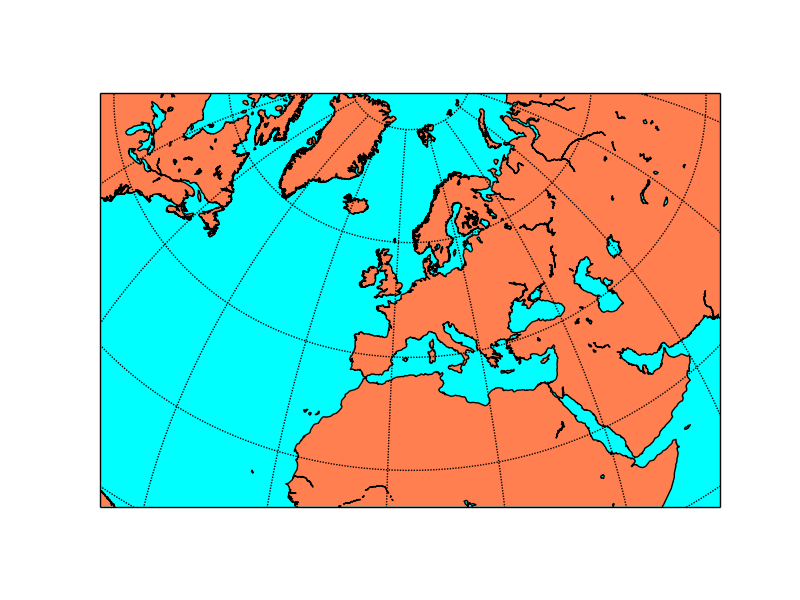
\includegraphics[scale=0.5,origin=c]{/Users/student/seminar/Kartendarstellungen/seminar/laea} \caption{Azimuthale flächentreue Lambert-Projektion}
\end{figure}
\newpage 